\documentclass{report}
\usepackage{graphicx} % Required for inserting images
\usepackage[utf8]{inputenc} % utf8 is recommended
\usepackage[T1]{fontenc} % T1 is recommended for Western languages
\usepackage{pgfplotstable}
\usepackage{booktabs} % For better table formatting
\usepackage{csvsimple} % For CSV file handling
\usepackage{longtable} % In case the table spans multiple pages
\usepackage{geometry}
\usepackage{lipsum}
\usepackage{tabularx}
\usepackage{hyperref}
\usepackage{ucs}
\usepackage{svg}
\usepackage{import}
\usepackage{xifthen}
\usepackage{pdfpages}
\usepackage[T1]{fontenc}
\usepackage[export]{adjustbox} 

\geometry{left=1in, right=1in, top=1in, bottom=1in} % set the margins

\title{\Huge\textbf{Navaho Linguistics for Quantum Hardware Education}\\
\author{\Large{Onri Jay Benally}}}
\date{December 2023}

\begin{document}

\maketitle


\large{This document is written by Onri Jay Benally, an Indigenous American born and raised on the Navaho tribe (Diné Bikeyah). Its purpose is to develop and collect Navaho terms associated with quantum information science and technology (QIST), highlighting on quantum hardware engineering. As you may find, this development is motivated by the drive not only to exploit linguistics as a way of better understanding emerging technology, but to also serve as a tool to contribute to the quantum community at large. With that, it may be possible to form a model around this effort in order to break down barriers to entry when it comes to approaching or incorporating oneself into the field of QIST. 
\\ 
\space
\\
\indent If you are interested in learning Navaho, the first section of this document will cover some basic ideas about the language. This will be followed by some examples of how one might think about names and labels from the Indigenous American perspective. It may be worth noting that although Navaho is considered to be a Tier 5 or Category 5 language in terms of difficulty for native English speakers, practicality is our main concern.
}


\begin{center}
\space
\end{center}


\begin{flushleft}
\title{\Large\textbf{Creative Commons License}}\\
\end{flushleft}

{
\large This work is licensed under the Creative Commons Attribution 4.0 International License. To view a copy of this license, visit \url{http://creativecommons.org/licenses/by/4.0/} or send a letter to Creative Commons, PO Box 1866, Mountain View, CA 94042, USA.
}

\begin{center}


\includegraphics{by.png}

\end{center}
\begin{center}
\Large\textbf{Towards Using Linguistics for Quantum Hardware Comprehension}
\end{center}

\large{
The Navaho language is highly descriptive, has a heavy presence of verb usage, and is rich in consonant clusters and tonality. It is important to note that the many biomes and topographical differences found on the tribal lands are contributing factors to the various Navaho dialects. This is especially true for the mountainous regions, where pronunciation and modern spelling can vary in a slight manner.
\\ 
\space
\\
\indent 
As you may or may not know, the Navaho language was only practiced through oral expression for thousands of years in what is now called North America. Not until relatively recent history did Navaho linguists and language experts decide to pick a written form that could adopt Navaho phonetics. So far, the Latin script (commonly used to write English alphabets) has been the default for writing since then. There are other scripts or writing systems such as Cyrillic (commonly used to write Slavic alphabets, including Russian) that can express Navaho phonetics as well, however it is not actively taught or practiced in the tribe. Either way, the spelling of words are expected to be pronounced phonetically.
\\ 
\space
\\
\indent 
For example, it is generally known that Diné has two English spellings: Navaho and Navajo (both pronounced the same). The letter (j), used in the word Navajo, is exclusive to the spelling of the word. If one observes (j) in any other Diné word, then it should be pronounced the same as the English letter (j) or its linearized form (dzh). Keep this in mind.
\\ 
\space
\\
\indent 
Virtually all English words can be translated into Navaho based on the depth of understanding and functionality of the word. Thus, when a new English term is coined or invented, a Navaho description can be given and verified by sharing it with another Navaho speaker who should understand what one is saying with context.
\\ 
\space
\\
\indent
In the era of rapidly advancing science, technology, and art, one can express new Navaho terms by simply spending some time to consider the semantics, followed by documenting or producing a shareable form of the new term. Such is the case for topics like quantum mechanics and quantum engineering, provided as examples in this repository. Over time, this documentation is expected to retain a fair amount of content for driving explanations of advanced and technical topics of today (especially quantum), in Navaho.
} 
% Be sure to move this curly bracket every time you create a new paragraph. %

\begin{center}
\Large\textbf{Towards a Model for Learning \& Using Navaho for Quantum Education}
\end{center}

\large{
• Find the root word.

• How does it behave?

• What is the historical relation?

• What is the suffix?

• What is the prefix?

• What are the particles, if any?

• Acknowledge that order doesn't matter that much inside the suffixes \& prefixes.
\\ 
\space
\\
For the original documentation:

• The quick brown fox jumped over the lazy dog, example in Navaho.

• Cyrillic example for "blue" in Navaho.

• Chart formation blueprint.

• Generate a table of Navaho characters in Unicode.

• Explore a draw-to-text for Navaho characters referencing Unicode.

• Label dilution refrigerator in Navaho.

• Label tunnel junctions \& physical qubit components in Navaho, may include original micrographs \& renderings in Blender.

• Potential contributions to Qiskit/ Qiskit Metal documentation in Navaho (from paper to GitHub pull requests).
\\ 
\space
\\
Note: Unicode is mentioned here due to its convenience of character generation when one desires to correctly spell Navaho words. This form of character generation may provide a robust sequence of protocols for practical language usage in digital form, further strengthening any future initiatives to automate Navaho translation.
\\ 
\space
\\
\indent
}
\begin{center}
\Large\textbf{Language Ideas for Quantum Hardware Comprehension}
\end{center}

\large{From idea to practice... 
\\ 
\space
\\

\begin{figure}[htbp]
    \centering
    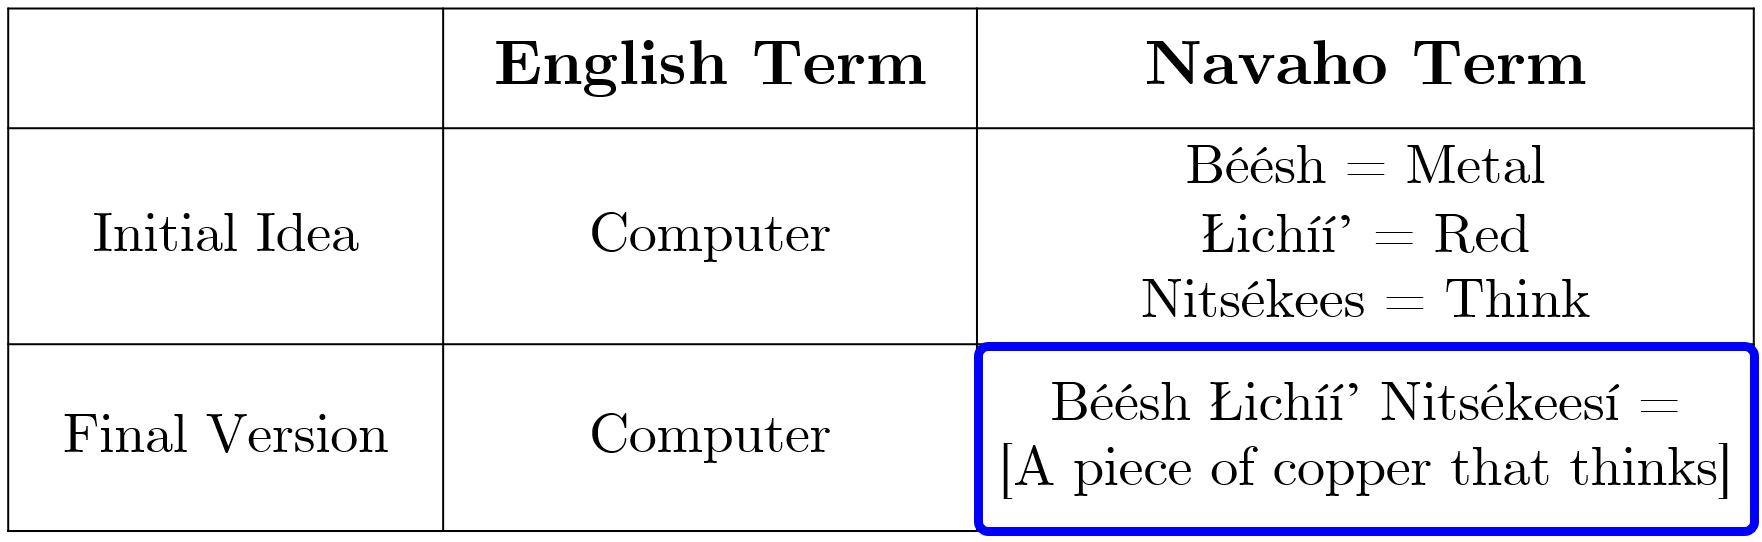
\includegraphics[width=0.9\textwidth]{Computer_NV.png}
    \caption{$Computer$ in Navaho.}
    \label{fig:svgImage}
\end{figure}

\large{
\noindent
Other examples:
\\ 
\space
\\
The quick brown fox = Ma'ii dibéłchíʼí tsį́įłgo or Ma'ii yishtłizh tsį́įłgo
\\ 
\space
\\
Lazy dog = léechąą’í iłhóyéé
\\ 
\space
\\
Jumped = nahachaʼ or dah nahachaʼ or dahnáníjįįh
\\ 
\space
\\
To jump = dahnáníshjį́į́h
\\ 
\space
\\
Jumping = dah nahácha’go
\\ 
\space
\\
Laziness = iłhóyéé
\\ 
\space
\\
Slow or in vain = chʼééh
\\ 
\space
\\
The quick brown fox jumped over the lazy dog = Ma'ii dibéłchíʼí tsį́įłgo léechąą’í iłhóyéé dahnáníjįįh
}
\begin{center}
\Large\textbf{Language Ideas for Quantum Hardware Comprehension}
\end{center}

\large{
\begin{figure}[htbp]
    \centering
    \includesvg[width=0.7\textwidth]{Navaho Vowel Network_v2.drawio.svg}
    \caption{Navaho long vowel network by Onri Jay Benally}
    \label{fig:svgImage}
\end{figure}
}
\begin{longtable}{|c|c|c|}
\hline
\textbf{Navaho Character} & \textbf{UTF-8 "U+" Notation} & \textbf{UTF-8 "\textbackslash{u}" Notation} \\
\hline
A & U+0041 & \textbackslash{}u0041 \\ \hline
B & U+0042 & \textbackslash{}u0042 \\ \hline
Ch' & U+0043 U+0068 U+0027 & \textbackslash{}u0043\textbackslash{}u0068\textbackslash{}u0027 \\ \hline
D & U+0044 & \textbackslash{}u0044 \\ \hline
Dl & U+0044 U+006C & \textbackslash{}u0044\textbackslash{}u006C \\ \hline
Dz & U+0044 U+007A & \textbackslash{}u0044\textbackslash{}u007A \\ \hline
E & U+0045 & \textbackslash{}u0045 \\ \hline
G & U+0047 & \textbackslash{}u0047 \\ \hline
Gh & U+0047 U+0068 & \textbackslash{}u0047\textbackslash{}u0068 \\ \hline
H & U+0048 & \textbackslash{}u0048 \\ \hline
Hw & U+0048 U+0077 & \textbackslash{}u0048\textbackslash{}u0077 \\ \hline
I & U+0049 & \textbackslash{}u0049 \\ \hline
J & U+004A & \textbackslash{}u004A \\ \hline
K & U+004B & \textbackslash{}u004B \\ \hline
K' & U+004B U+0027 & \textbackslash{}u004B\textbackslash{}u0027 \\ \hline
Kw & U+004B U+0077 & \textbackslash{}u004B\textbackslash{}u0077 \\ \hline
L & U+004C & \textbackslash{}u004C \\ \hline
Ł & U+0141 & \textbackslash{}u0141 \\ \hline
M & U+004D & \textbackslash{}u004D \\ \hline
N & U+004E & \textbackslash{}u004E \\ \hline
O & U+004F & \textbackslash{}u004F \\ \hline
S & U+0053 & \textbackslash{}u0053 \\ \hline
Sh & U+0053 U+0068 & \textbackslash{}u0053\textbackslash{}u0068 \\ \hline
T & U+0054 & \textbackslash{}u0054 \\ \hline
T' & U+0054 U+0027 & \textbackslash{}u0054\textbackslash{}u0027 \\ \hline
Tł & U+0054 U+0142 & \textbackslash{}u0054\textbackslash{}u0142 \\ \hline
Tł' & U+0054 U+0142 U+0027 & \textbackslash{}u0054\textbackslash{}u0142\textbackslash{}u0027 \\ \hline
Ts & U+0054 U+0073 & \textbackslash{}u0054\textbackslash{}u0073 \\ \hline
Ts' & U+0054 U+0073 U+0027 & \textbackslash{}u0054\textbackslash{}u0073\textbackslash{}u0027 \\ \hline
W & U+0057 & \textbackslash{}u0057 \\ \hline
X & U+0058 & \textbackslash{}u0058 \\ \hline
Y & U+0059 & \textbackslash{}u0059 \\ \hline
Z & U+005A & \textbackslash{}u005A \\ \hline

aa & U+0061 U+0061 & \textbackslash{}u0061\textbackslash{}u0061 \\ \hline
á & U+00E1 & \textbackslash{}u00E1 \\ \hline
áá & U+00E1 U+00E1 & \textbackslash{}u00E1\textbackslash{}u00E1 \\ \hline
ą & U+0105 & \textbackslash{}u0105 \\ \hline
ąą & U+0105 U+0105 & \textbackslash{}u0105\textbackslash{}u0105 \\ \hline
ą́ & U+0105 U+0301 & \textbackslash{}u0105\textbackslash{}u0301 \\ \hline
ą́ą́ & U+0105 U+0301 U+0105 U+0301 & \textbackslash{}u0105\textbackslash{}u0301\textbackslash{}u0105\textbackslash{}u0301 \\ \hline

aá & U+0061 U+00E1 & \textbackslash{}u0061\textbackslash{}u00E1 \\ \hline
aą & U+0061 U+0105 & \textbackslash{}u0061\textbackslash{}u0105 \\ \hline
aą́ & U+0061 U+0105 U+0301 & \textbackslash{}u0061\textbackslash{}u0105\textbackslash{}u0301 \\ \hline

áa & U+00E1 U+0061  & \textbackslash{}u00E1\textbackslash{}u0061 \\ \hline
áą & U+00E1 U+0105 & \textbackslash{}u00E1\textbackslash{}u0105 \\ \hline
áą́ & U+00E1 U+0105 U+0301 & \textbackslash{}u00E1\textbackslash{}u0105\textbackslash{}u0301 \\ \hline

ąa & U+0105 U+0061  & \textbackslash{}u0105\textbackslash{}u0061 \\ \hline
ąá & U+0105 U+00E1 & \textbackslash{}u0105\textbackslash{}u00E1 \\ \hline
ąą́ & U+0105 U+0105 U+0301  & \textbackslash{}u0105\textbackslash{}u0105\textbackslash{}u0301 \\ \hline

ą́a & U+0105 U+0301 U+0061 & \textbackslash{}u0105\textbackslash{}u0301\textbackslash{}u0061 \\ \hline
ą́á & U+0105 U+0301 U+00E1 & \textbackslash{}u0105\textbackslash{}u0301\textbackslash{}u00E1 \\ \hline
ą́ą & U+0105 U+0301 U+0105 & \textbackslash{}u0105\textbackslash{}u0301\textbackslash{}u0105 \\ \hline

ee & U+0065 U+0065 & \textbackslash{}u0065\textbackslash{}u0065 \\ \hline
é & U+00E9 & \textbackslash{}u00E9 \\ \hline
éé & U+00E9 U+00E9 & \textbackslash{}u00E9\textbackslash{}u00E9 \\ \hline
ę & U+0119 & \textbackslash{}u0119 \\ \hline
ęę & U+0119 U+0119 & \textbackslash{}u0119\textbackslash{}u0119 \\ \hline
ę́ & U+0119 U+0301 & \textbackslash{}u0119\textbackslash{}u0301 \\ \hline
ę́ę́ & U+0119 U+0301 U+0119 U+0301 & \textbackslash{}u0119\textbackslash{}u0301\textbackslash{}u0119\textbackslash{}u0301 \\ \hline

eé & U+0065 U+00E9 & \textbackslash{}u0065\textbackslash{}u00E9 \\ \hline
eę & U+0065 U+0119 & \textbackslash{}u0065\textbackslash{}u0119 \\ \hline
eę́ & U+0065 U+0119 U+0301 & \textbackslash{}u0065\textbackslash{}u0119\textbackslash{}u0301 \\ \hline

ée & U+00E9 U+0065 & \textbackslash{}u00E9\textbackslash{}u0065 \\ \hline
éę & U+00E9 U+0119 & \textbackslash{}u00E9\textbackslash{}u0119 \\ \hline
éę́ & U+00E9 U+0119 U+0301 & \textbackslash{}u00E9\textbackslash{}u0119\textbackslash{}u0301 \\ \hline

ęe & U+0119 U+0065 & \textbackslash{}u0119\textbackslash{}u0065 \\ \hline
ęé & U+0119 U+00E9  & \textbackslash{}u0119\textbackslash{}u00E9 \\ \hline
ęę́ & U+0119 U+0119 U+0301 & \textbackslash{}u0119\textbackslash{}u0119\textbackslash{}u0301 \\ \hline

ę́e & U+0119 U+0301 U+0065 & \textbackslash{}u0119\textbackslash{}u0301\textbackslash{}u0065 \\ \hline
ę́ę & U+0119 U+0301 U+0119 & \textbackslash{}u0119\textbackslash{}u0301\textbackslash{}u0119 \\ \hline
ę́é & U+0119 U+0301 U+00E9  & \textbackslash{}u0119\textbackslash{}u0301\textbackslash{}u00E9 \\ \hline

ii & U+0069 U+0069  & \textbackslash{}u0069\textbackslash{}u0069 \\ \hline
í & U+00ED & \textbackslash{}u00ED \\ \hline
íí & U+00ED U+00ED & \textbackslash{}u00ED\textbackslash{}u00ED \\ \hline
į & U+012F & \textbackslash{}u012F \\ \hline
įį & U+012F U+012F & \textbackslash{}u012F\textbackslash{}u012F \\ \hline
į́ & U+012F U+0301 & \textbackslash{}u012F\textbackslash{}u0301 \\ \hline
į́į́ & U+012F U+0301 U+012F U+0301 & \textbackslash{}u012F\textbackslash{}u0301\textbackslash{}u012F\textbackslash{}u0301 \\ \hline

ií & U+0069 U+00ED & \textbackslash{}u0069\textbackslash{}u00ED \\ \hline
iį & U+0069 U+012F & \textbackslash{}u0069\textbackslash{}u012F \\ \hline
iį́ & U+0069 U+012F U+0301 & \textbackslash{}u0069\textbackslash{}u012F\textbackslash{}u0301 \\ \hline

íi & U+00ED U+0069 & \textbackslash{}u00ED\textbackslash{}u0069 \\ \hline
íį & U+00ED U+012F  & \textbackslash{}u00ED\textbackslash{}u012F \\ \hline
íį́ & U+00ED U+012F U+0301 & \textbackslash{}u00ED\textbackslash{}u012F\textbackslash{}u0301 \\ \hline

įi & U+012F U+0069 & \textbackslash{}u012F\textbackslash{}u0069 \\ \hline
įí & U+012F U+00ED & \textbackslash{}u012F\textbackslash{}u00ED \\ \hline
įį́ & U+012F U+012F U+0301 & \textbackslash{}u012F\textbackslash{}u012F\textbackslash{}u0301 \\ \hline

į́i & U+012F U+0301 U+0069 & \textbackslash{}u012F\textbackslash{}u0301\textbackslash{}u0069 \\ \hline
į́í & U+012F U+0301 U+00ED & \textbackslash{}u012F\textbackslash{}u0301\textbackslash{}u00ED \\ \hline
į́į & U+012F U+0301 U+012F & \textbackslash{}u012F\textbackslash{}u0301\textbackslash{}u012F \\ \hline

oo &  U+006F  U+006F & \textbackslash{}u006F\textbackslash{}u006F \\ \hline
ó & U+00F3 & \textbackslash{}u00F3 \\ \hline
óó & U+00F3 U+00F3 & \textbackslash{}u00F3\textbackslash{}u00F3 \\ \hline
ǫ & U+01EB & \textbackslash{}u01EB \\ \hline
ǫǫ & U+01EB U+01EB & \textbackslash{}u01EB\textbackslash{}u01EB \\ \hline
ǫ́ & U+01EB U+0301 & \textbackslash{}u01EB\textbackslash{}u0301 \\ \hline
ǫ́ǫ́ & U+01EB U+0301 U+01EB U+0301 & \textbackslash{}u01EB\textbackslash{}u0301\textbackslash{}u01EB\textbackslash{}u0301 \\ \hline

oó &  U+006F U+00F3 & \textbackslash{}u006F\textbackslash{}u00F3 \\ \hline
oǫ &  U+006F U+01EB & \textbackslash{}u006F\textbackslash{}u00EB \\ \hline
oǫ́ &  U+006F U+01EB U+0301 & \textbackslash{}u006F\textbackslash{}u01EB\textbackslash{}u0301 \\ \hline

óo & U+00F3 U+006F & \textbackslash{}u00F3\textbackslash{}u006F \\ \hline
óǫ & U+00F3 U+01EB & \textbackslash{}u00F3\textbackslash{}u01EB \\ \hline
óǫ́ & U+00F3 U+01EB U+0301 & \textbackslash{}u00F3\textbackslash{}u01EB\textbackslash{}u0301 \\ \hline

ǫo & U+01EB U+006F  & \textbackslash{}u01EB\textbackslash{}u006F \\ \hline
ǫó & U+01EB U+00F3 & \textbackslash{}u01EB\textbackslash{}u00F3 \\ \hline
ǫǫ́ & U+01EB U+01EB U+0301 & \textbackslash{}u01EB\textbackslash{}u01EB\textbackslash{}u0301 \\ \hline

ǫ́o & U+01EB U+0301 U+006F & \textbackslash{}u01EB\textbackslash{}u0301\textbackslash{}u006F \\ \hline
ǫ́ǫ & U+01EB U+0301 U+01EB & \textbackslash{}u01EB\textbackslash{}u0301\textbackslash{}u01EB \\ \hline
ǫ́ó & U+01EB U+0301 U+00F3 & \textbackslash{}u01EB\textbackslash{}u0301\textbackslash{}u00F3 \\ \hline

ń & U+0144 & \textbackslash{}u0144 \\ \hline
\end{longtable}

\begin{longtable}{|c|c|c|}
\hline
Navaho Character & UTF-8 "U+" Notation & UTF-8 "\textbackslash{u}" Notation \\
\hline
A & U+0041 & \textbackslash{}u0041 \\ \hline
B & U+0042 & \textbackslash{}u0042 \\ \hline
Ch' & U+0043 U+0068 U+0027 & \textbackslash{}u0043\textbackslash{}u0068\textbackslash{}u0027 \\ \hline
D & U+0044 & \textbackslash{}u0044 \\ \hline
Dl & U+0044 U+006C & \textbackslash{}u0044\textbackslash{}u006C \\ \hline
Dz & U+0044 U+007A & \textbackslash{}u0044\textbackslash{}u007A \\ \hline
E & U+0045 & \textbackslash{}u0045 \\ \hline
G & U+0047 & \textbackslash{}u0047 \\ \hline
Gh & U+0047 U+0068 & \textbackslash{}u0047\textbackslash{}u0068 \\ \hline
H & U+0048 & \textbackslash{}u0048 \\ \hline
Hw & U+0048 U+0077 & \textbackslash{}u0048\textbackslash{}u0077 \\ \hline
I & U+0049 & \textbackslash{}u0049 \\ \hline
J & U+004A & \textbackslash{}u004A \\ \hline
K & U+004B & \textbackslash{}u004B \\ \hline
K' & U+004B U+0027 & \textbackslash{}u004B\textbackslash{}u0027 \\ \hline
Kw & U+004B U+0077 & \textbackslash{}u004B\textbackslash{}u0077 \\ \hline
L & U+004C & \textbackslash{}u004C \\ \hline
Ł & U+0141 & \textbackslash{}u0141 \\ \hline
M & U+004D & \textbackslash{}u004D \\ \hline
N & U+004E & \textbackslash{}u004E \\ \hline
O & U+004F & \textbackslash{}u004F \\ \hline
S & U+0053 & \textbackslash{}u0053 \\ \hline
Sh & U+0053 U+0068 & \textbackslash{}u0053\textbackslash{}u0068 \\ \hline
T & U+0054 & \textbackslash{}u0054 \\ \hline
T' & U+0054 U+0027 & \textbackslash{}u0054\textbackslash{}u0027 \\ \hline
Tł & U+0054 U+0142 & \textbackslash{}u0054\textbackslash{}u0142 \\ \hline
Tł' & U+0054 U+0142 U+0027 & \textbackslash{}u0054\textbackslash{}u0142\textbackslash{}u0027 \\ \hline
Ts & U+0054 U+0073 & \textbackslash{}u0054\textbackslash{}u0073 \\ \hline
Ts' & U+0054 U+0073 U+0027 & \textbackslash{}u0054\textbackslash{}u0073\textbackslash{}u0027 \\ \hline
W & U+0057 & \textbackslash{}u0057 \\ \hline
X & U+0058 & \textbackslash{}u0058 \\ \hline
Y & U+0059 & \textbackslash{}u0059 \\ \hline
Z & U+005A & \textbackslash{}u005A \\ \hline

aa & U+0061 U+0061 & \textbackslash{}u0061\textbackslash{}u0061 \\ \hline
á & U+00E1 & \textbackslash{}u00E1 \\ \hline
áá & U+00E1 U+00E1 & \textbackslash{}u00E1\textbackslash{}u00E1 \\ \hline
ą & U+0105 & \textbackslash{}u0105 \\ \hline
ąą & U+0105 U+0105 & \textbackslash{}u0105\textbackslash{}u0105 \\ \hline
ą́ & U+0105 U+0301 & \textbackslash{}u0105\textbackslash{}u0301 \\ \hline
ą́ą́ & U+0105 U+0301 U+0105 U+0301 & \textbackslash{}u0105\textbackslash{}u0301\textbackslash{}u0105\textbackslash{}u0301 \\ \hline

aá & U+0061 U+00E1 & \textbackslash{}u0061\textbackslash{}u00E1 \\ \hline
aą & U+0061 U+0105 & \textbackslash{}u0061\textbackslash{}u0105 \\ \hline
aą́ & U+0061 U+0105 U+0301 & \textbackslash{}u0061\textbackslash{}u0105\textbackslash{}u0301 \\ \hline

áa & U+00E1 U+0061  & \textbackslash{}u00E1\textbackslash{}u0061 \\ \hline
áą & U+00E1 U+0105 & \textbackslash{}u00E1\textbackslash{}u0105 \\ \hline
áą́ & U+00E1 U+0105 U+0301 & \textbackslash{}u00E1\textbackslash{}u0105\textbackslash{}u0301 \\ \hline

ąa & U+0105 U+0061  & \textbackslash{}u0105\textbackslash{}u0061 \\ \hline
ąá & U+0105 U+00E1 & \textbackslash{}u0105\textbackslash{}u00E1 \\ \hline
ąą́ & U+0105 U+0105 U+0301  & \textbackslash{}u0105\textbackslash{}u0105\textbackslash{}u0301 \\ \hline

ą́a & U+0105 U+0301 U+0061 & \textbackslash{}u0105\textbackslash{}u0301\textbackslash{}u0061 \\ \hline
ą́á & U+0105 U+0301 U+00E1 & \textbackslash{}u0105\textbackslash{}u0301\textbackslash{}u00E1 \\ \hline
ą́ą & U+0105 U+0301 U+0105 & \textbackslash{}u0105\textbackslash{}u0301\textbackslash{}u0105 \\ \hline

ee & U+0065 U+0065 & \textbackslash{}u0065\textbackslash{}u0065 \\ \hline
é & U+00E9 & \textbackslash{}u00E9 \\ \hline
éé & U+00E9 U+00E9 & \textbackslash{}u00E9\textbackslash{}u00E9 \\ \hline
ę & U+0119 & \textbackslash{}u0119 \\ \hline
ęę & U+0119 U+0119 & \textbackslash{}u0119\textbackslash{}u0119 \\ \hline
ę́ & U+0119 U+0301 & \textbackslash{}u0119\textbackslash{}u0301 \\ \hline
ę́ę́ & U+0119 U+0301 U+0119 U+0301 & \textbackslash{}u0119\textbackslash{}u0301\textbackslash{}u0119\textbackslash{}u0301 \\ \hline

eé & U+0065 U+00E9 & \textbackslash{}u0065\textbackslash{}u00E9 \\ \hline
eę & U+0065 U+0119 & \textbackslash{}u0065\textbackslash{}u0119 \\ \hline
eę́ & U+0065 U+0119 U+0301 & \textbackslash{}u0065\textbackslash{}u0119\textbackslash{}u0301 \\ \hline

ée & U+00E9 U+0065 & \textbackslash{}u00E9\textbackslash{}u0065 \\ \hline
éę & U+00E9 U+0119 & \textbackslash{}u00E9\textbackslash{}u0119 \\ \hline
éę́ & U+00E9 U+0119 U+0301 & \textbackslash{}u00E9\textbackslash{}u0119\textbackslash{}u0301 \\ \hline

ęe & U+0119 U+0065 & \textbackslash{}u0119\textbackslash{}u0065 \\ \hline
ęé & U+0119 U+00E9  & \textbackslash{}u0119\textbackslash{}u00E9 \\ \hline
ęę́ & U+0119 U+0119 U+0301 & \textbackslash{}u0119\textbackslash{}u0119\textbackslash{}u0301 \\ \hline

ę́e & U+0119 U+0301 U+0065 & \textbackslash{}u0119\textbackslash{}u0301\textbackslash{}u0065 \\ \hline
ę́ę & U+0119 U+0301 U+0119 & \textbackslash{}u0119\textbackslash{}u0301\textbackslash{}u0119 \\ \hline
ę́é & U+0119 U+0301 U+00E9  & \textbackslash{}u0119\textbackslash{}u0301\textbackslash{}u00E9 \\ \hline

ii & U+0069 U+0069  & \textbackslash{}u0069\textbackslash{}u0069 \\ \hline
í & U+00ED & \textbackslash{}u00ED \\ \hline
íí & U+00ED U+00ED & \textbackslash{}u00ED\textbackslash{}u00ED \\ \hline
į & U+012F & \textbackslash{}u012F \\ \hline
įį & U+012F U+012F & \textbackslash{}u012F\textbackslash{}u012F \\ \hline
į́ & U+012F U+0301 & \textbackslash{}u012F\textbackslash{}u0301 \\ \hline
į́į́ & U+012F U+0301 U+012F U+0301 & \textbackslash{}u012F\textbackslash{}u0301\textbackslash{}u012F\textbackslash{}u0301 \\ \hline

ií & U+0069 U+00ED & \textbackslash{}u0069\textbackslash{}u00ED \\ \hline
iį & U+0069 U+012F & \textbackslash{}u0069\textbackslash{}u012F \\ \hline
iį́ & U+0069 U+012F U+0301 & \textbackslash{}u0069\textbackslash{}u012F\textbackslash{}u0301 \\ \hline

íi & U+00ED U+0069 & \textbackslash{}u00ED\textbackslash{}u0069 \\ \hline
íį & U+00ED U+012F  & \textbackslash{}u00ED\textbackslash{}u012F \\ \hline
íį́ & U+00ED U+012F U+0301 & \textbackslash{}u00ED\textbackslash{}u012F\textbackslash{}u0301 \\ \hline

įi & U+012F U+0069 & \textbackslash{}u012F\textbackslash{}u0069 \\ \hline
įí & U+012F U+00ED & \textbackslash{}u012F\textbackslash{}u00ED \\ \hline
įį́ & U+012F U+012F U+0301 & \textbackslash{}u012F\textbackslash{}u012F\textbackslash{}u0301 \\ \hline

į́i & U+012F U+0301 U+0069 & \textbackslash{}u012F\textbackslash{}u0301\textbackslash{}u0069 \\ \hline
į́í & U+012F U+0301 U+00ED & \textbackslash{}u012F\textbackslash{}u0301\textbackslash{}u00ED \\ \hline
į́į & U+012F U+0301 U+012F & \textbackslash{}u012F\textbackslash{}u0301\textbackslash{}u012F \\ \hline

oo &  U+006F  U+006F & \textbackslash{}u006F\textbackslash{}u006F \\ \hline
ó & U+00F3 & \textbackslash{}u00F3 \\ \hline
óó & U+00F3 U+00F3 & \textbackslash{}u00F3\textbackslash{}u00F3 \\ \hline
ǫ & U+01EB & \textbackslash{}u01EB \\ \hline
ǫǫ & U+01EB U+01EB & \textbackslash{}u01EB\textbackslash{}u01EB \\ \hline
ǫ́ & U+01EB U+0301 & \textbackslash{}u01EB\textbackslash{}u0301 \\ \hline
ǫ́ǫ́ & U+01EB U+0301 U+01EB U+0301 & \textbackslash{}u01EB\textbackslash{}u0301\textbackslash{}u01EB\textbackslash{}u0301 \\ \hline

oó &  U+006F U+00F3 & \textbackslash{}u006F\textbackslash{}u00F3 \\ \hline
oǫ &  U+006F U+01EB & \textbackslash{}u006F\textbackslash{}u00EB \\ \hline
oǫ́ &  U+006F U+01EB U+0301 & \textbackslash{}u006F\textbackslash{}u01EB\textbackslash{}u0301 \\ \hline

óo & U+00F3 U+006F & \textbackslash{}u00F3\textbackslash{}u006F \\ \hline
óǫ & U+00F3 U+01EB & \textbackslash{}u00F3\textbackslash{}u01EB \\ \hline
óǫ́ & U+00F3 U+01EB U+0301 & \textbackslash{}u00F3\textbackslash{}u01EB\textbackslash{}u0301 \\ \hline

ǫo & U+01EB U+006F  & \textbackslash{}u01EB\textbackslash{}u006F \\ \hline
ǫó & U+01EB U+00F3 & \textbackslash{}u01EB\textbackslash{}u00F3 \\ \hline
ǫǫ́ & U+01EB U+01EB U+0301 & \textbackslash{}u01EB\textbackslash{}u01EB\textbackslash{}u0301 \\ \hline

ǫ́o & U+01EB U+0301 U+006F & \textbackslash{}u01EB\textbackslash{}u0301\textbackslash{}u006F \\ \hline
ǫ́ǫ & U+01EB U+0301 U+01EB & \textbackslash{}u01EB\textbackslash{}u0301\textbackslash{}u01EB \\ \hline
ǫ́ó & U+01EB U+0301 U+00F3 & \textbackslash{}u01EB\textbackslash{}u0301\textbackslash{}u00F3 \\ \hline

ń & U+0144 & \textbackslash{}u0144 \\ \hline
\end{longtable}


\end{document}
